\documentclass{beamer}


\usepackage{amsmath}
\usepackage{amsthm}
\usepackage{amsfonts}

\usepackage{accents}
\usepackage{graphicx}
\def\b{\begin}
\def\e{\end}
\def\tb{\textbf}
\def\p{\partial}
\def\CC{\mathbb{C}}
\def\f{\frac}
\def\RR{\mathbb{R}}


\theoremstyle{plain}
\newtheorem{prop}{Proposition}
\newtheorem{thm}{Theorem}[section]
\newtheorem{claim}{Claim}
\newtheorem{lem}[thm]{Lemma}

\theoremstyle{definition}
\newtheorem{dfn}{Definition}[section]




\begin{document}

\title{\textbf{Rogue Waves in the Nonlinear Schr\"{o}dinger Equation}}
\author{\textsc{by Andy Reagan}}
\date{May 11, 2012}


\frame{\maketitle}



\section[Outline]{}
\frame{\tableofcontents}

\section{Introduction}

\frame
{
\begin{figure}
\begin{center}
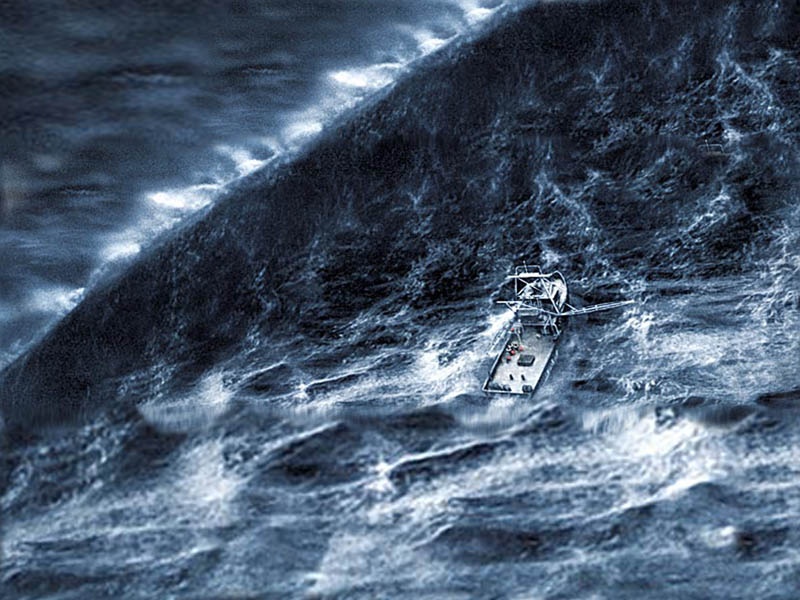
\includegraphics[width=200px]{perfect-storm.jpeg}\\
Figure 0: Rogue wave?
\end{center}
\end{figure}
\vspace{-1mm}
}

\frame
{
\begin{figure}
\begin{center}
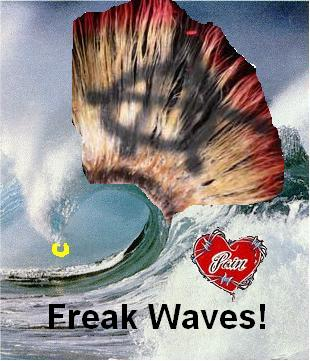
\includegraphics[width=200px]{reardon.JPG}\\
Figure 1: Definitely rogue
\end{center}
\end{figure}
\vspace{-1mm}
}

\frame
{
\begin{figure}
\begin{center}
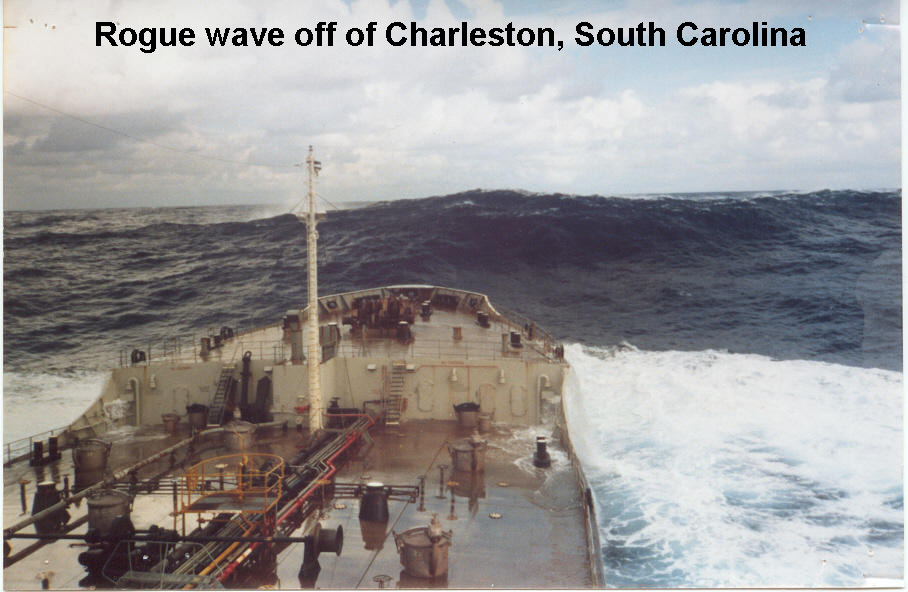
\includegraphics[width=200px]{rogue_wave2.jpg}\\
Figure 2: Observed rogue wave
\end{center}
\end{figure}
\vspace{-1mm}
}
  
  
  \frame
{
\begin{figure}
\begin{center}
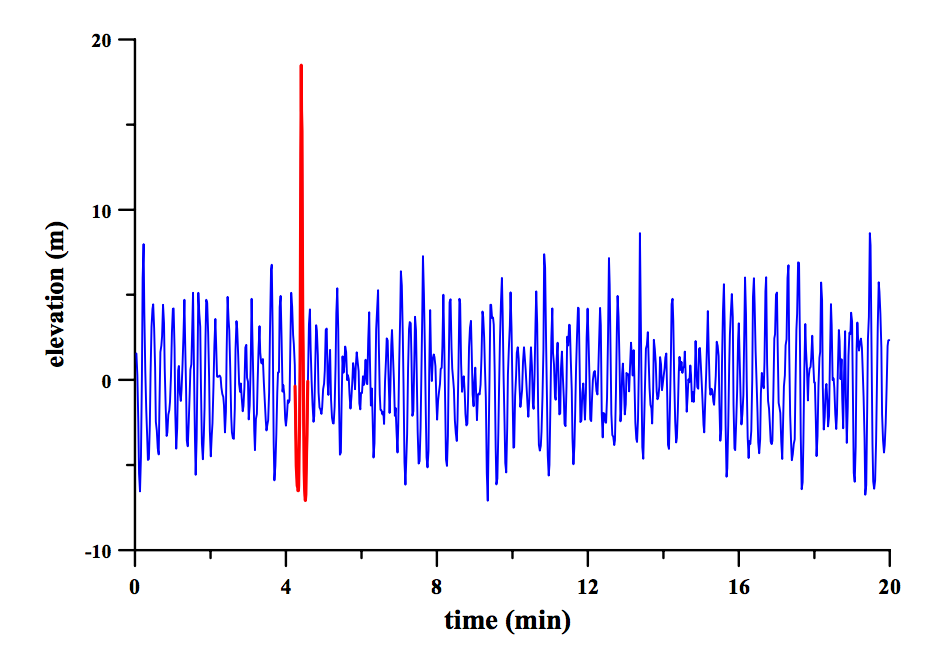
\includegraphics[width=200px]{draupner_wave.png}\\
Figure 3: The "Draupner Wave"
\end{center}
\end{figure}
\vspace{-1mm}
}
  

\frame{  
\frametitle{What are rogue waves}
\b{itemize}

\item Once considered to be a mythical occurrence, rogue waves are now a studied phenomenon in nonlinear wave  theory. \\[25pt]

\pause
\item The structure and nature of these waves is imperative in our understanding of how and why they occur.\\[25pt]

\pause
\item Occur in both water and optical waves.
\e{itemize}
}

\frame
{
\b{itemize}
\item In oceanography, the pragmatic approach is to 
define a rogue wave whenever
\begin{equation*}\tag{1.1}
H/H_s>2\quad\text{or}\quad\omega_c/H_s>1.25
\e{equation*}
where $H$ is the wave height (distance from trough to crest), $\omega_c$ is the crest height (distance from mean sea level to crest), and $H_s$ is the significant wave height, here defined as four times the standard deviation of the surface elevation.  

\pause
\item Known to cause extensive damage, and are even life-threatening, when they come into contact with ocean liners and passenger ships in the open waters.  

\pause
\item Between 1964 and 1994, it is estimated that more than 22 super-carriers have been lost at sea as a direct result of rogue waves (Kharif \& Pelinovsky 2003).
\e{itemize}
}

\frame
{
\frametitle{Physical mechanisms of rogue wave formation}
\b{itemize}

\item Normal part of wave spectrum\\[25pt]

\pause
\item Linear and non-linear spatial focusing\\[25pt]

\pause
\item Wave-current interaction\\[25pt]

\pause
\item Non-linear modulation instability

%\item Recently, there has been the discovery of a similar wave phenomenon observed in optics\\[10pt]
%\item A growing consensus is that both oceanic and optical rogue waves appear as a result of modulation instability of monochromatic nonlinear waves (Ohta \& Yang 2012). \\[10pt]
%\item As a result, we must turn to mathematically studying these waves thus we turn our attention to an integrable model, the nonlinear Schr\"{o}dinger (NLS) (Zakharov \& Shabat 1967). 
\e{itemize}
}

\frame
{\b{itemize}
\item Standard soliton wave solutions approach zero as time goes to $\pm\infty$ whereas rogue wave solutions approach a nonzero constant as time goes to $\pm\infty$, with the first analytical solution obtained by Peregrine (1983). \\[10pt]

\pause
\item Ohta and Yang (2012) derived general high-order waves in the NLS equation using the bilinear method in the soliton theory, and then further simplified there results to algebraic expressions using Gram determinants and elementary Schur polynomials.  

\e{itemize}
}

%\frame
%{
%\begin{dfn}Let $V$ be an inner product space over a field $k$ with $<\cdot,\cdot>$ the inner product on $V$, where the inner product shall mean a symmetric bilinear form on $V$.  Let $x_1,x_2,\ldots,x_n$ be arbitrary vectors in $V$. Set $r_{ij}=<x_i,x_j>$. The Gram determinant of $x_1,x_2,\ldots,x_n$ is determined to be the determinant of the symmetric matrix
%\begin{equation*}\tag{1.2}
%\begin{pmatrix}
%r_{11}& \cdots & r_{1n}\\
%\vdots& \ddots & \vdots\\
%r_{n1} & \cdots & r_{nn}
%\e{pmatrix}.
%\e{equation*}
%
%\e{dfn}
%}

\frame
{
\begin{dfn} Let $S_n(\boldsymbol x)$ be the elementary Schur polynomial defined by the generating function
\begin{equation*}\tag{1.3}
\sum_{n=0}^{\infty}S_n(\boldsymbol x)\lambda^n=\exp\left(\sum_{n=0}^{\infty}x_k\lambda^k\right),
\e{equation*}
where $\boldsymbol x=(x_1,x_2,\ldots)$. Such that the first few terms are
\begin{equation*}
S_0(\boldsymbol x)=1,\quad S_1(\boldsymbol x)=1,\quad S_2(\boldsymbol x)=\frac{1}{2}x_{1}^2+x_2,\quad S_3(\boldsymbol x)=\frac{1}{6}x_{1}^3+x_1x_2+x_3,\, \ldots
\e{equation*}
\e{dfn}
}

%\frame
%{
%The purpose of this paper will be to reproduce the main results of Ohta and Yang (2012), and extend the numerical methods to higher-order solutions.  The derivations will also be based on the bilinear method in soliton theory \cite{hirota2004}, which will then be expanded to general rogue waves of $N$-th order with $N-1$ free parameters, using Gram determinants, which will be numerically simulated using a program created by the authors with Mathematica.
%}

\section{General Rogue-Wave Solutions of the NLS}
\frame
{
If we consider the general rogue wave solutions of the focusing NLS equation
\begin{equation*}\tag{2.1}
iu_t=u_{xx}+2|u|^2u
\e{equation*}
we find it is invariant under scalings $x\rightarrow\alpha x$, $t\rightarrow\alpha^2t$, $u\rightarrow u/\alpha$ for any constant $\alpha\in\mathbb{R}$, as well as the Galilean transformation $u(x,t)\rightarrow u(x-vt,t)\exp(-ivx/2+iv^2t/4)$ (Ohta \& Yang 2012).
Therefore, we will consider the rogue waves that approach a nonzero constant background at large $x$ and $t$,
\begin{equation*}
u(x,t)\rightarrow e^{-2it}\quad\text{as}\quad x,\,t\rightarrow\pm\infty.
\e{equation*}
}

\frame
{
If we apply the variable transformation $u\rightarrow ue^{-2it}$, then (2.1) becomes
\begin{equation*}\tag{2.2}
\begin{aligned}
i(ue^{-2it})_t&=(ue^{-2it})_{xx}+2\left|ue^{-2it}\right|^2\cdot ue^{-2it}\\
i\left(u_te^{-2it}-2iue^{-2it}\right)&=e^{-2it}u_{xx}+2|u|^2\cdot ue^{-2it}\\
iu_te^{-2it}&=e^{-2it}u_{xx}+2|u|^2\cdot ue^{-2it}-2ue^{-2it}\\
iu_t&=u_{xx}+2u\left(|u|^2-1\right)
\e{aligned}
\e{equation*}
where the boundary conditions become
\begin{equation*}\tag{2.3}
u(x,t)\rightarrow 1\quad\text{as}\quad x,\,t\rightarrow\pm\infty.
\e{equation*}
}

%\frame
%{

%Since the Schur polynomials give the complete set of homogenous-weight algebraic solutions for the Kadomstev-Petviashvili (KP) hierarchy (Sata 1981; Jimbo \& Miwa 1983), we can also use them to describe the rational solutions of rogue waves in the NLS equation (Ohta \& Yang 2012).
%}

\frame
{
\frametitle{Main result}
The NLS equation (2.1) under the boundary conditions (2.3) has non-singular rational solutions
\begin{equation*}
u=\dfrac{\sigma_1}{\sigma_0}
\e{equation*}
where
\begin{equation*}
\sigma_n=\det_{1\le i,j\le N}\left(m^{(n)}_{2i-1,j-1}\right).
\e{equation*}
The matrix elements in $\sigma_m$ are defined by
\begin{equation*}
\begin{aligned}
m_{ij}^{(n)}&=\sum_{v=0}^{\min(i,j)}\Phi_{iv}^{(n)}\Psi_{jv}^{(n)} .
\e{aligned}
\e{equation*}
}

\frame
{
\frametitle{Main result, contd}
Where
\begin{equation*}
\Phi_{iv}^{(n)}=\dfrac{1}{2^v}\sum^{i-v}_{k=0}a_kS_{i-v-k}\left(\boldsymbol x^{+}(n)+vs\right)\end{equation*}
\begin{equation*}
\Psi_{jv}^{(n)}=\dfrac{1}{2^v}\sum^{j-v}_{l=0}\overline{a}_lS_{j-v-l}\left(\boldsymbol x^{-}(n)+vs\right)
\e{equation*}
for $a_k$ for $k=0,1,\ldots$ are complex constants, and $\boldsymbol x^{\pm}(n)=(x_1^{\pm}(n),\ldots)$, $\boldsymbol s=(s_1,lots)$ are defined by 
\begin{equation*}\tag{2.4}
x_1^{\pm}(n)=x\mp2it\pm n-\dfrac{1}{2},\quad x_k^{\pm}=\dfrac{x\mp2^kit}{k!}-r_k, \quad(k\ge2),
\e{equation*}
and
\begin{equation*}
\sum^{\infty}_{k=1}r_k\lambda^k=\ln\left(\cosh\dfrac{\lambda}{2}\right)\quad\text{and}\quad\sum^{\infty}_{k=1}s_k\lambda^k=\ln\left(\dfrac{2}{\lambda}\tanh\dfrac{\lambda}{2}\right).
\e{equation*}
}

%\frame
%{
%\frametitle{Main Theorem,contd}
%Here we have $\overline{a}_l$ is the complex conjugate of $a_l$.  Therefore, $\sigma^n$ can be expressed by
%\begin{equation*}
%\sigma^n=\sum^{1}_{v_1=0}\sum^{3}_{v_2=v_1+1}\sum^{5}_{v_3=v_2+1}\cdots\sum^{2N-1}_{v_N=v_{N-1}+1}\det_{1\le i,j\le N}\left(\Phi^{(n)}_{2i-1,v_j}\right)\det_{1\le i,j\le N}\left(\Psi^{(n)}_{2i-1,v_j}\right)
%\e{equation*}
%such that
%\begin{equation*}
%\Phi^{(n)}_{iv}\quad\text{and}\quad\Psi^{(n)}_{iv}\quad\text{for}\quad i<v.
%\e{equation*}
%}

%\frame
%{
%\frametitle{Generating $r_k, s_k$}
%
%Demo
%
%}


\subsection{Deriving Bilinear Form}
\frame 
{
\frametitle{Deriving Bilinear Form}
First we derive the bilinear form of the transformed NLS from (2.1). Let $u=g/f$ for $g\in \CC, f\in \RR$. Then we have
\begin{align*} 0 & = \left ( \f{g}{f} \right ) _{xx} + 2 \left ( \left | \f{g}{f} \right | ^2 - 1 \right ) \f{g}{f} - i \left ( \f{g}{f} \right ) _t \\
& = \left ( \f{fg_x -gf_x }{f^2} \right ) _x + 2 \left ( \f{|g|^2g}{f^3} -\f{g}{f} \right ) - i \left ( \f{fg_t-gf_t}{f^2} \right ) \\
& = \f{f^2(fg_{xx}-gf_{xx}) - (fg_x -gf_x)2f}{f^4} + 2 \left ( \f{|g|^2g}{f^3} -\f{g}{f} \right )- i \left ( \f{fg_t-gf_t}{f^2} \right ). \end{align*}
}

\frame
{
By multiplying through by $f^3$, and then grouping by $g,f$ we have
\begin{align*} 0 & = f(f_{xx}-gf_{xx}) - 2 (fg_x -gf_x) + 2 |g|^2 g - gf^2 -if(fg_t-gf_t)\\&= f((fg_{xx} -gf_{xx} ) -i (fg_t -gf_t) ) + g\left ( 2|g|^2 -f^2-2f\f{g_x}{g} -2f_x \right ) \\
& = f(D_x^2 -iD_t)(gf) + g((D_x^2 +2)(f^2)) - 2|g|^2)
\end{align*}
}

\frame
{
so we have the desired bilinear form 

\begin{equation*}\tag{3.1}
 \left. \begin{array}{rl} (D_x ^2 + 2) f\cdot f & = 2|g|^2 \\ \text{and} ~~ (D_x^2 - iD_t) g\cdot f & = 0, \end{array} \right \}
 \e{equation*} 
where $D$ is Hirota's bilinear differential operator such that $D_x (fg) = f_xg - g_xf.$
Then for $h$ another complex variable, we consider the $2+1$-dimensional generalization of the above bilinear form 
\begin{equation*}\tag{3.2}
 \left. \begin{array}{rl} (D_x D_y + 2) f\cdot f&= 2gh \\ \text{and} ~~ (D_x^2 - iD_t) g\cdot f&= 0. \end{array} \right \}
 \e{equation*} 
}

\frame
{

Solutions to equations (3.2) under the conditions
\begin{equation*}\tag{3.3}
(\partial _x + \partial _y)f = Cf, ~~~~~~~~~~\text{where}\quad f\in\RR\quad\text{and}\quad h=\overline{g}
\end{equation*}
for $C$ some constant then also satisfy the bilinear NLS equations, since then $gh=|g|^2$ and $D_xD_y (f) = D_x ^2 (f)$.

Next, we verify Lemma 3.1 of Ohta and Yang (2012) to begin constructing Gram determinant solutions to the $2+1$-dimensional bilinear system.
}

\subsection{Gram determinant solutions to 2+1 dimensional bilinear equations}

\frame
{
\frametitle{Lemma} Let $m_{ij}^{(n)}, \phi _i ^{(n)} , \psi _j ^{(n)}$ be functions of $x_1 , x_2, x_{-1}$ satisfying the following differential and difference relations, $$ \left. \begin{array}{rl} \partial _{x_1} m_{ij} ^{(n)} & = \phi _i ^{(n)} \psi _j ^{(n)} ,\\
\partial _{x_2} m_{ij} ^{(n)} & = \phi _i ^{(n+1)} \psi _j ^{(n)} + \phi _i ^{(n)} \psi ^{(n-1)} ,\\
\partial _{x_{-1} } m_{ij} ^{(n)} & = -\phi _i ^{(n-1)} \psi _j ^{(n+1)},\\
m _{ij} ^{(n+1)} & = m_{ij} ^{(n)} + \phi _i ^{(n)} \psi _j ^{(n+1)} ,\\
\text{and}~~~~~\partial _{x_k} \phi _i ^{(n)} & = \phi _i ^{(n+k)}, ~~\partial _{x_k} \psi _j ^{(n)}=-\psi _j ^{(n-k)}, ~(k=1,2,-1). \end{array} \right \} $$
}

\frame
{
\frametitle{Lemma, contd} 
Then the determinant, $$\tau _n = \det _{1\leq i,j \leq N} \left ( m_{ij} ^{(n)} \right ),$$ satisfies the bilinear equations,
$$ \left. \begin{array}{rl} ( D_{x_1} D_{x_{-1}} -2 ) \tau _n \cdot \tau _n & = -2 \tau _{n+1} \tau _{n-1}\\
\text{and} ~(D_{x_1} ^2 - D_{x_2} ) \tau _{n+1} \cdot \tau _n & = 0 . \end{array} \right \} $$
}

\frame
{
\emph{Proof.} We then verify
\begin{align*} \partial _{x_1} \tau _n & = \left | \begin{array}{cc} m_{ij} ^{(n)} & \phi _i ^{(n)} \\ - \psi _j ^{(n)} & 0 \end{array} \right | ,\\
\partial _{x_1} ^2 \tau _n & = \left | \begin{array}{cc} m_{ij} ^{(n)} & \phi _i ^{(n+1)} \\ - \phi _j ^{(n)} & 0 \end{array} \right | + \left | \begin{array}{cc} m_{ij} ^{(n)} & \phi _i ^{(n)} \\ \phi _j ^{(n-1)} & 0 \end{array} \right | ,\\
\partial _{x_2} \tau _n & = \left | \begin{array}{cc} m_{ij} ^{(n)} & \phi _i ^{(n+1)} \\ - \phi _j ^{(n)} & 0 \end{array} \right | - \left | \begin{array}{cc} m_{ij} ^{(n)} & \phi _i ^{(n)} \\ \phi _j ^{(n-1)} & 0 \end{array} \right | ,\\
& \vdots \end{align*}
}

\frame
{
So we have \begin{align*} (\partial _{x_1} \partial _{x_{-1}} - 1) \tau _n \times \tau _n & = \partial _{x_1} \tau _n \times \partial _{x_{-1}} \tau _n - ( - \tau _{n-1} )(-\tau _{n+1}) ,\\
\tfrac{1}{2} (\partial _{x_1} ^2 - \partial _{x_2} ) \tau _{n+1} \times \tau _n  & = \partial _{x_1} \tau _{n+1} \times \partial _{x_1} \tau _n  - \tau _{n+1} \tfrac{1}{2} (\partial _{x_1} ^2 + \partial _{x_2} ) \tau _n , \end{align*}
which is the bilinear form of the $2+1$-dimensional NLS, as desired. \qed\\
}

\frame
{
Since we write $$ m_{ij} ^{(n)} = \int ^{x_1} \phi _i ^{(n)} \psi _j ^{(n)} dx_1 $$ the determinant $\tau _n$ is the Gram determinant solution. By defining 
\begin{equation*}\tag{3.11}
f= \tau _0, ~~~g=\tau _1 ,~~~h=\tau _{-1},
\end{equation*}
these are the Gram determinant solutions for the $2+1$-dimensional bilinear system where
\begin{equation*}\tag{3.12}
x_1=x,\,x_2=-it,\,\text{and}\,x_{-1}=-y.
\e{equation*}

The following Lemma shows that by choosing the matrix elements appropriately in $\tau _n$, we have solutions that also satisfy the reduction condition.
}


%
\subsection{Algebraic solutions satisfying reduction condition}



\frame
{
\frametitle{Lemma}
Define matrix elements $$\left . m_{ij} ^{(n)} = A_i B_j m ^{(n)} \right | _{p=1,q=1}$$ and $$m^{(n)} = \f{1}{p+q} \left ( - \f{p}{q} \right ) ^n e ^{\xi +\eta } , ~~~\xi = px_1 + p^2 x_2, ~~~\eta = q x_1 - q^2 x_2 , $$ where $A_i,B_j$ are differential operators with respect to $p,q$ defined as 
\begin{align*} A_0 & = a_0,\\ A_1&  = a_0 p \partial _p + a_1,\\ A_2 & = \f{a_0}{2} (p \partial _p ) ^2 + a_1 p \partial _p + a_2, \\ & \vdots \end{align*} 
}

\frame
{
\frametitle{Lemma, contd}
\begin{align*} B_0 & = b_0,\\ B_1&  = b_0 q \partial _q + b_1,\\ B_2 & = \f{b_0}{2} (q \partial _q ) ^2 + b_1 q \partial _q + b_2, \\ & \vdots \end{align*} 
where $a_k,b_l$ are constants.  Then the determinant $$ \tau _n = \det _{1 \leq i,j \leq N } ( m^{(n)} _{2i-1,2j-1} ) = \left | \begin{array}{ccc} m _{1,1} ^{(n)} & \cdots & m _{1,2N-1} ^{(n)}\\ \vdots & \ddots & \vdots \\ m _{2N-1,1} ^{(n)} & \cdots & m _{2N-1,2N-1} ^{(n)} \end{array} \right | $$ satisfies the NLS bilinear equations. 
}

\subsection{Complex Conjugacy and Simplification of Rogue-Wave Solutions}

\frame
{
%The proof to Lemma 3.2 is too long for this presentation, and can be found in Ohta and Yang (2012). 

If we combine the complex conjugate conditions of (3.3) with (3.11) we have that 
\begin{equation*}\tag{3.31}
\tau_0\in\mathbb{R} \quad\text{and}\quad\tau_{-1}=\overline{\tau}_1\in\CC.
\end{equation*}
Thus combining (3.31) with (3.12), we can satisfy the above condition by taking the parameters $a_k$ and $b_k$ of Lemma 3.2 to be complex conjugates of one another such that $b_k=\overline{a}_k$. With this condition in mind we know that the rational solution from the main result is non-singular since $u=g/f=\tau_1/\tau_0$ where $f=\tau_0$.% is the determinant of a positive definite matrix and therefore $f>0$.
}

%\frame
%{
%We can then simplify the rogue-wave solutions such that if we take the generator $\mathcal{G}$ of the differential operators $(p\partial_p)^k(q\partial_q)^l$ defined by
%\begin{align*} \tag{3.32}
%\mathcal{G} & =\sum_{k=0}^{\infty}\sum_{l=0}^{\infty}\dfrac{\kappa^k}{k!}\dfrac{\lambda^l}{l!}(p\partial_p)^k(q\partial_q)^l\\&=\exp(\kappa p\partial_p+\lambda q \partial q)=\exp(\kappa\partial_{\ln p}+\lambda\partial_{\ln q})
%\end{align*}
%then for any function $F(p,q)$, we have
%\begin{equation*}\tag{3.33}
%\mathcal{G}F(p,q)=F(e^{\kappa}p,e^{\lambda}q)
%\e{equation*}
%}

%\frame
%{
%such that expanding the right-hand side of (3.33) into a Taylor series of $(\kappa,\lambda)$ around the point $(0,0)$, rewriting the exponent in terms of $x^+_k$ and $x^-_l$ as defined in (2.4), calculating the matrix element of the Gram determinant, $\sigma_n$, and applying the Laplace expansion to the determinant we are left with rational solutions of the form of Theorem 2.1 (Ohta \& Yang 2012). 
%}

\section{Numerical Simulations of Rogue-Wave Solutions}

\frame
{
\begin{figure}[h]
\begin{center}
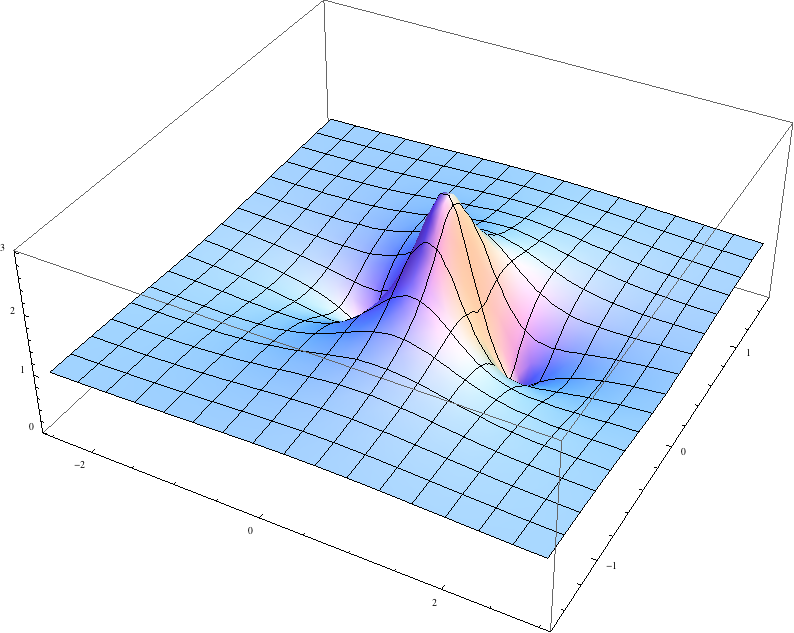
\includegraphics[width=200px]{1st_order.png}\\
Figure 4: Mathematica plot of 1st order rogue wave solution.
\end{center}
\end{figure}
\vspace{-1mm}
}

\frame
{
\begin{figure}
\begin{center}
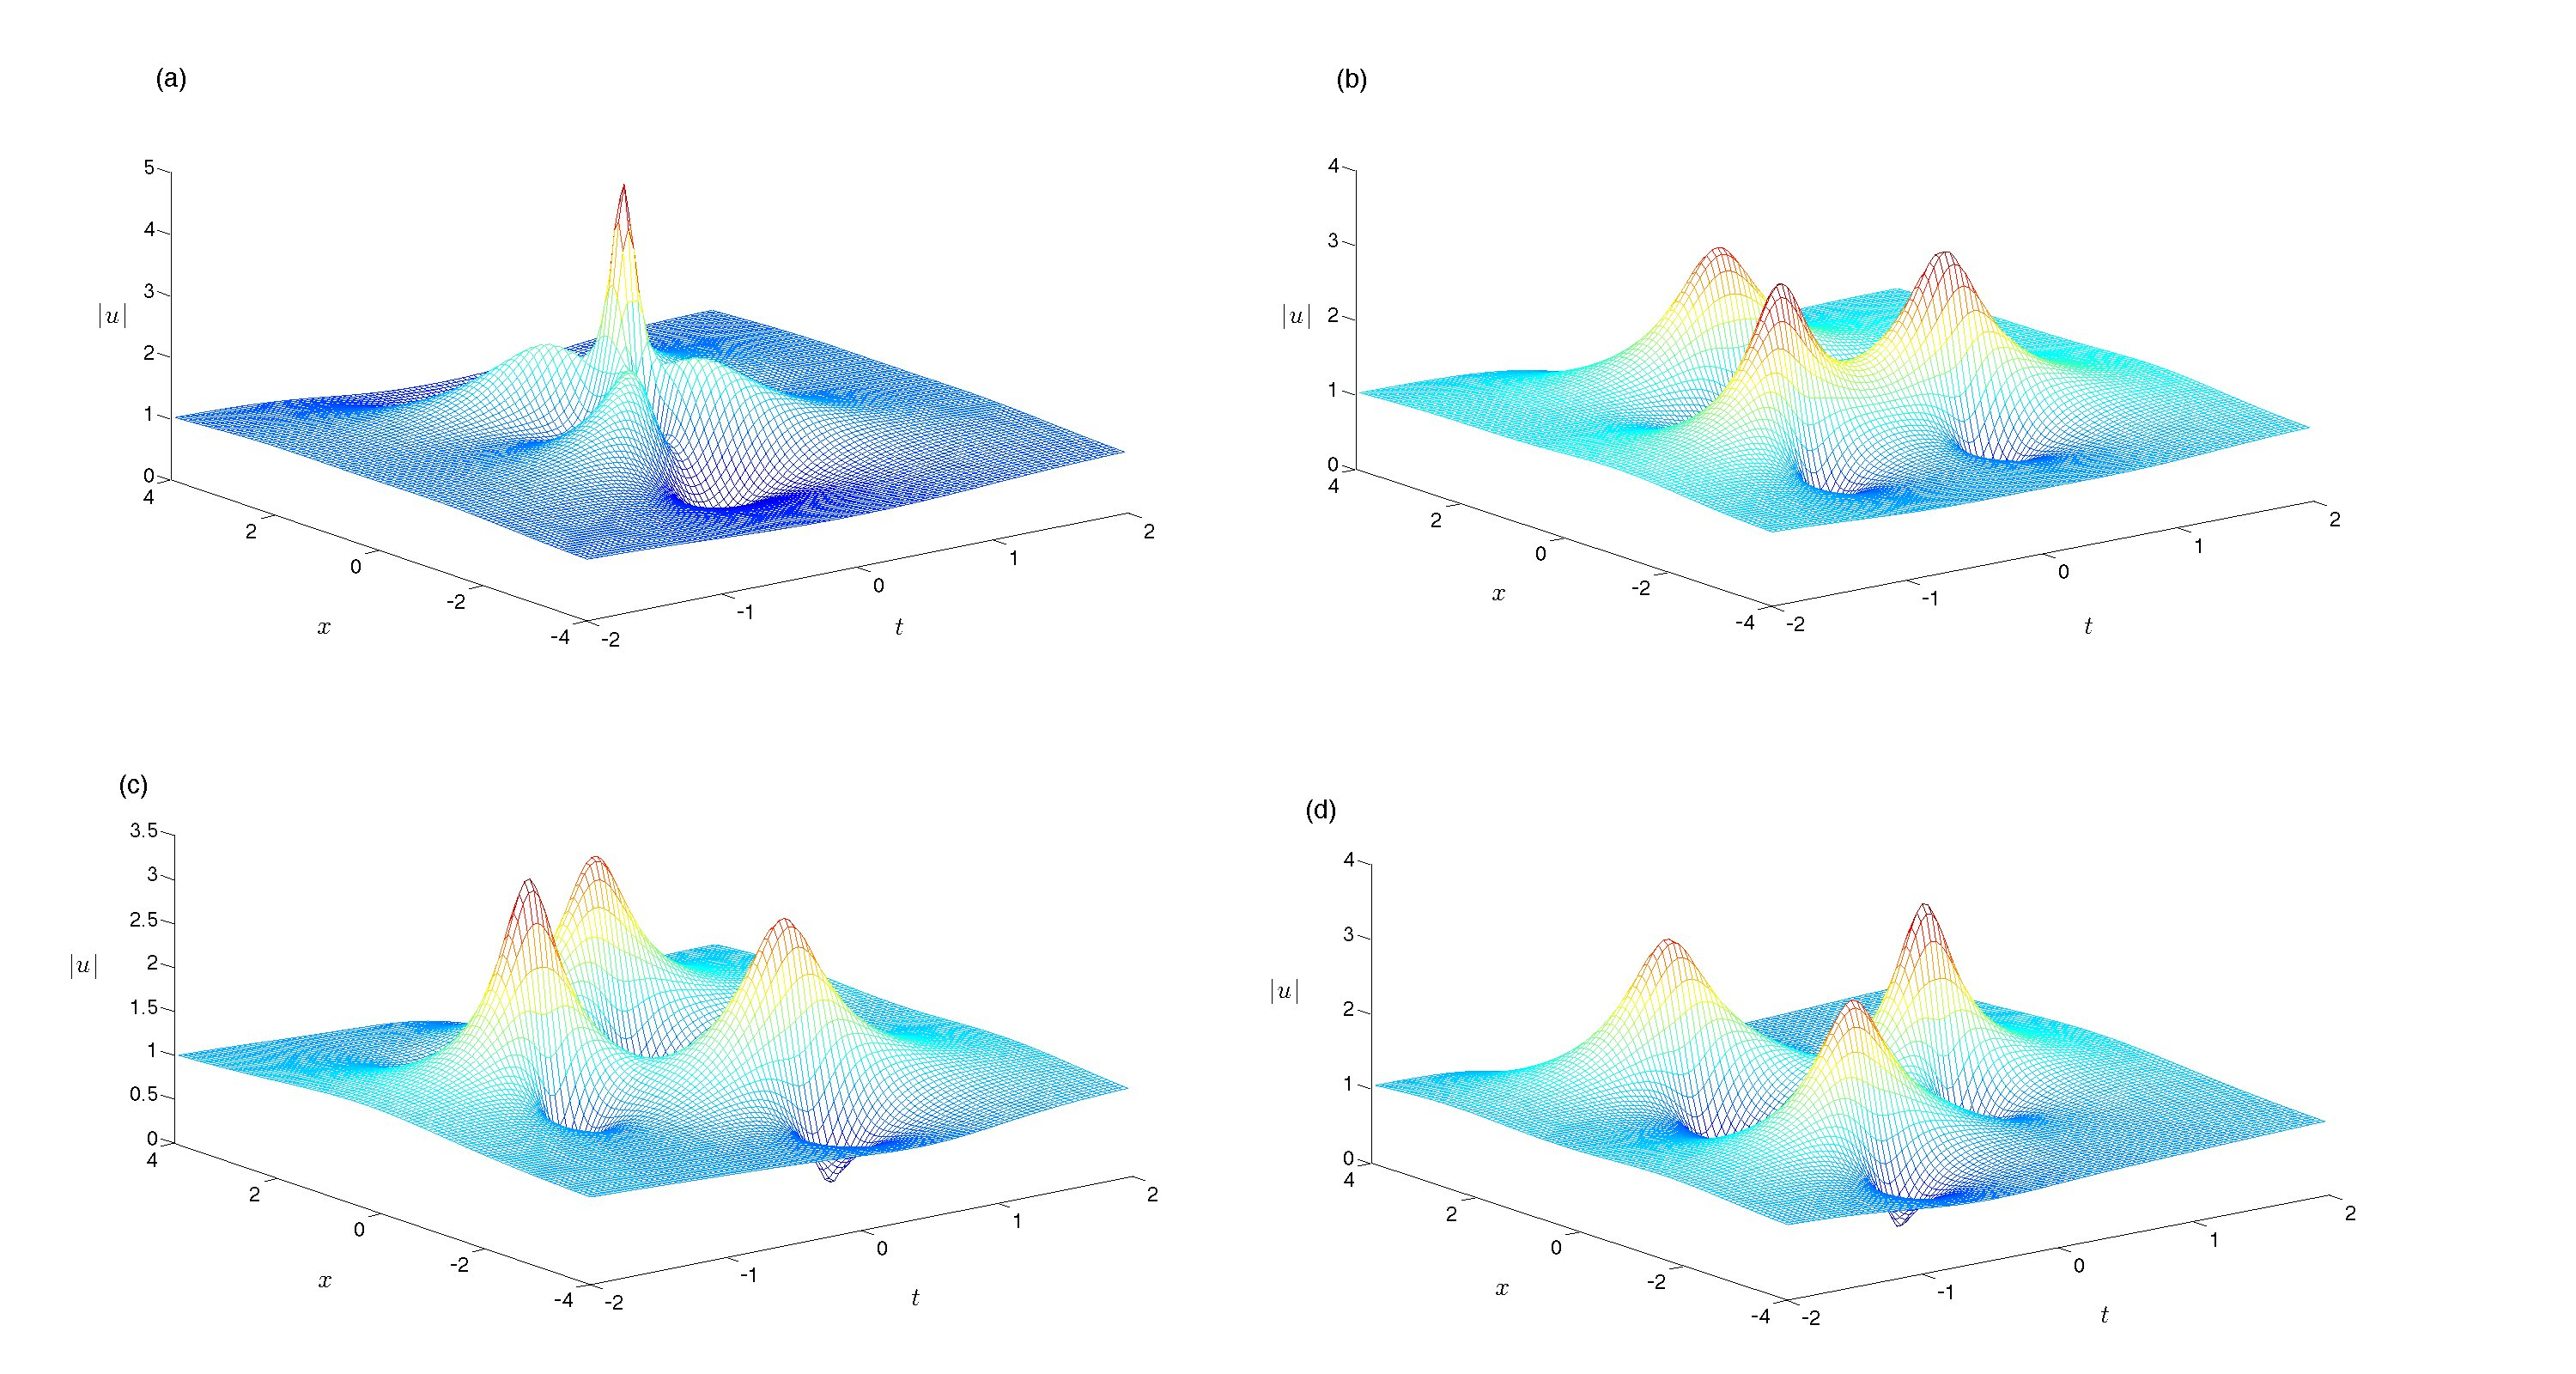
\includegraphics[width=280px]{figure1_new.jpg}\\
Figure 5: 2nd order wave solutions plotted in MATLAB for the following values of $a_3$: (a) -1/12, (b) 5/3, (c) $-5i/2$, and (d) $5i/2$.
\end{center}
\end{figure}
}

\frame
{
\vspace{0mm}
\begin{figure}
\begin{center}
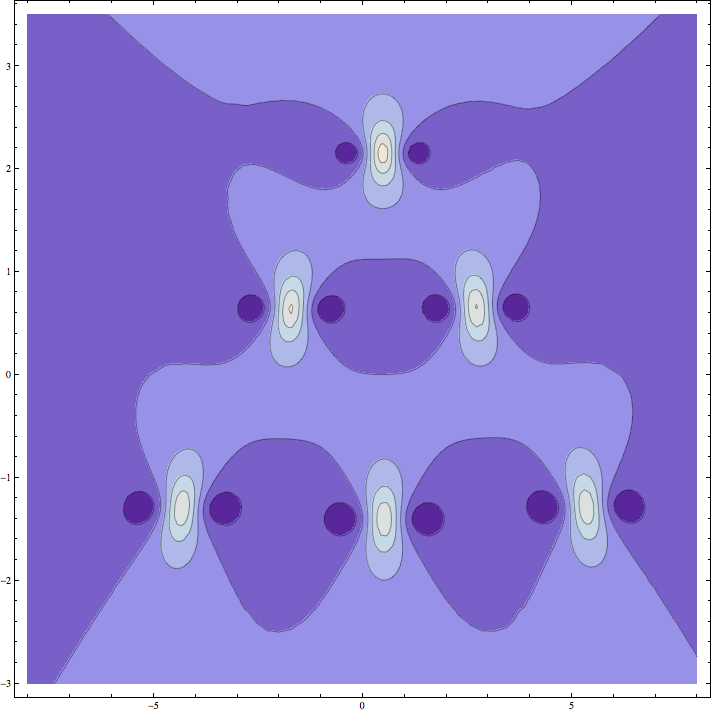
\includegraphics[width=150px]{3rd_order_many_peaks_contour.png}\\
Figure 6: Mathematica contour plot of 3rd order solution for $(a_3,a_5)=(25i/3,0)$ showing 6 intensity humps.
\end{center}
\end{figure}
}

\frame
{
\begin{figure}
\begin{center}
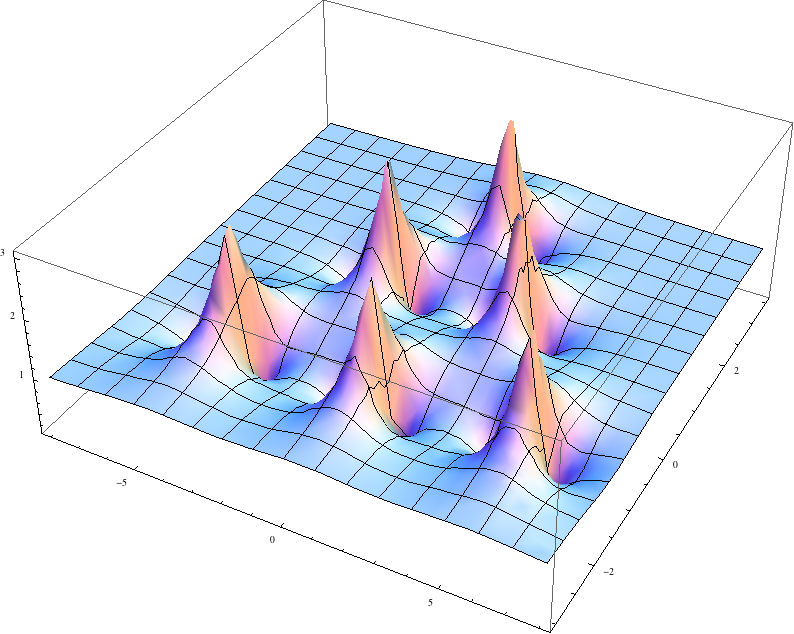
\includegraphics[width=200px]{3rd_order_many_peaks.png}\\
Figure 7: Mathematica plot of 3rd order solution for $(a_3,a_5)=(25i/3,0)$.
\end{center}
\end{figure}
\vspace{-1mm}
}

\frame
{
\begin{figure}
\begin{center}
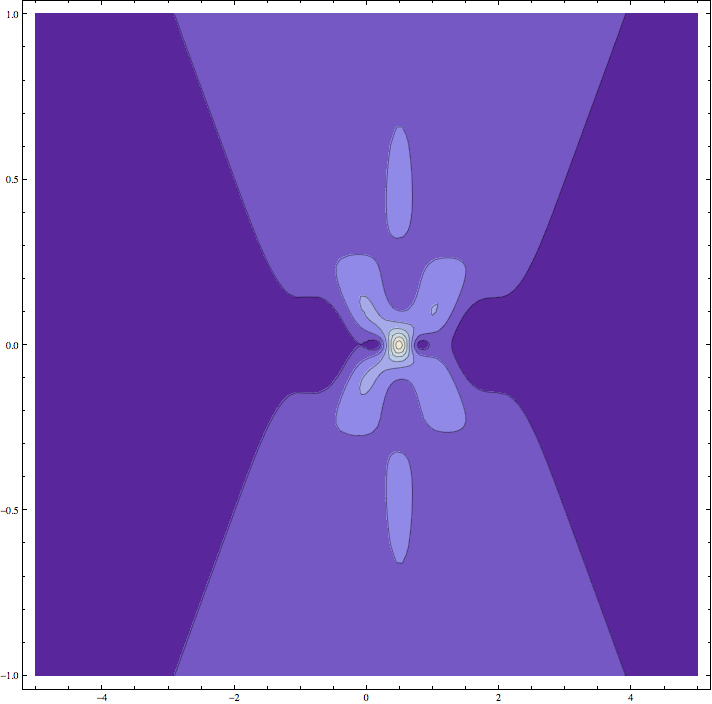
\includegraphics[width=150px]{3rd_order_max_peak_contour.png}\\
Figure 8: Mathematica contour plot of 3rd order solution for $(a_3,a_5)=(-1/12,-1/240)$ which achieves a maximum amplitude of 9 at $(x,t)=(1/2,0)$.
\end{center}
\end{figure}
\vspace{-1mm}
}

\frame
{
\begin{figure}
\begin{center}
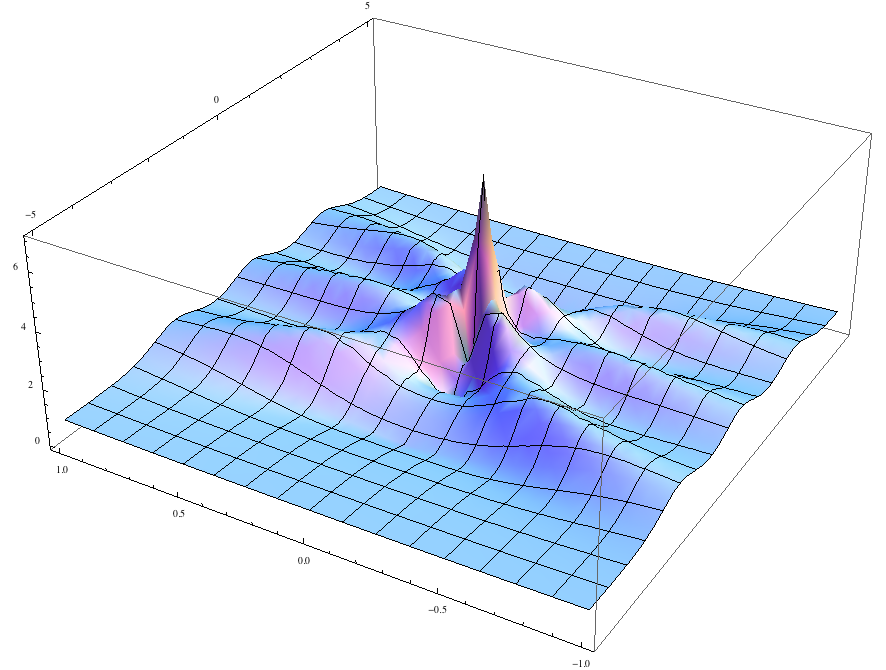
\includegraphics[width=200px]{3rd_order_max_peak.png}\\
Figure 9:  Mathematica plot of 3rd order solution for $(a_3,a_5)=(-1/12,-1/240)$.
\end{center}
\end{figure}
\vspace{-1mm}
}

\frame{
\begin{figure}
\begin{center}
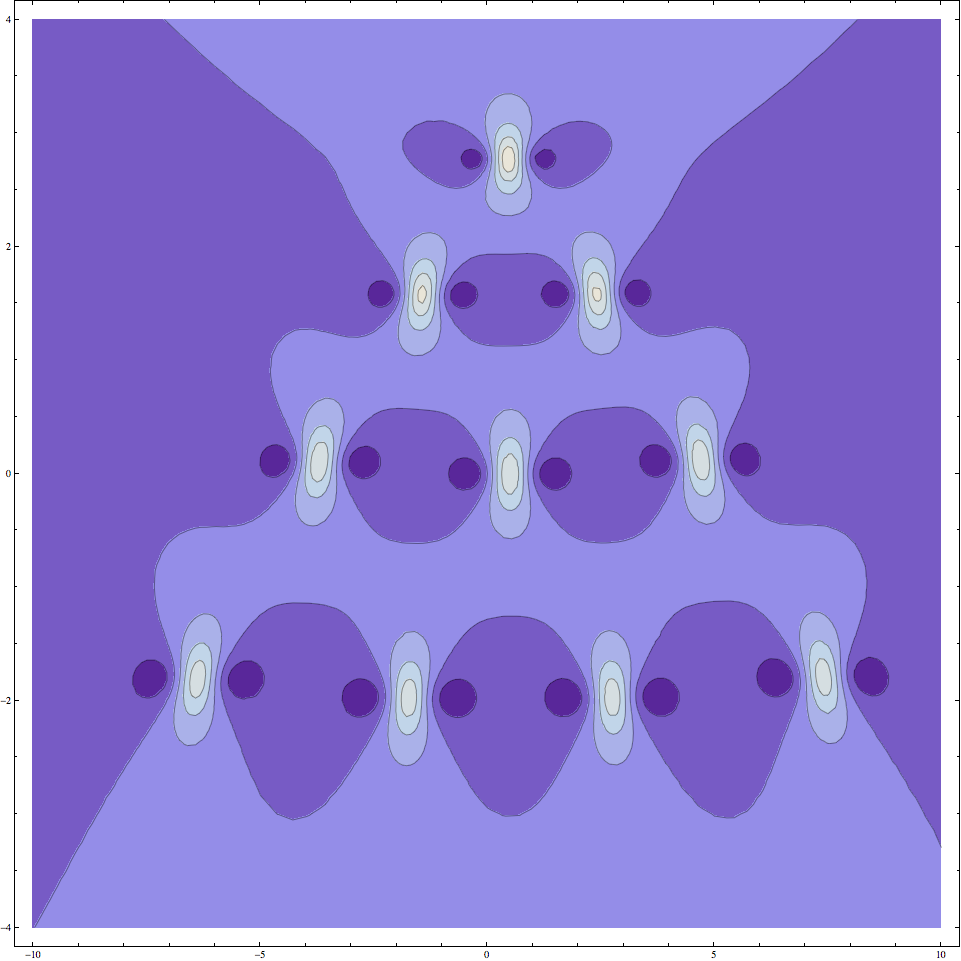
\includegraphics[width=150px]{4th_order_many_peaks_contour.png}\\
Figure 10: Mathematica contour plot of 4rd order solution for $(a_3,a_5,a_7)=(25i/3,0,0)$ showing 10 intensity humps.
\end{center}
\end{figure}
\vspace{-1mm}
}

\frame
{
\begin{figure}
\begin{center}
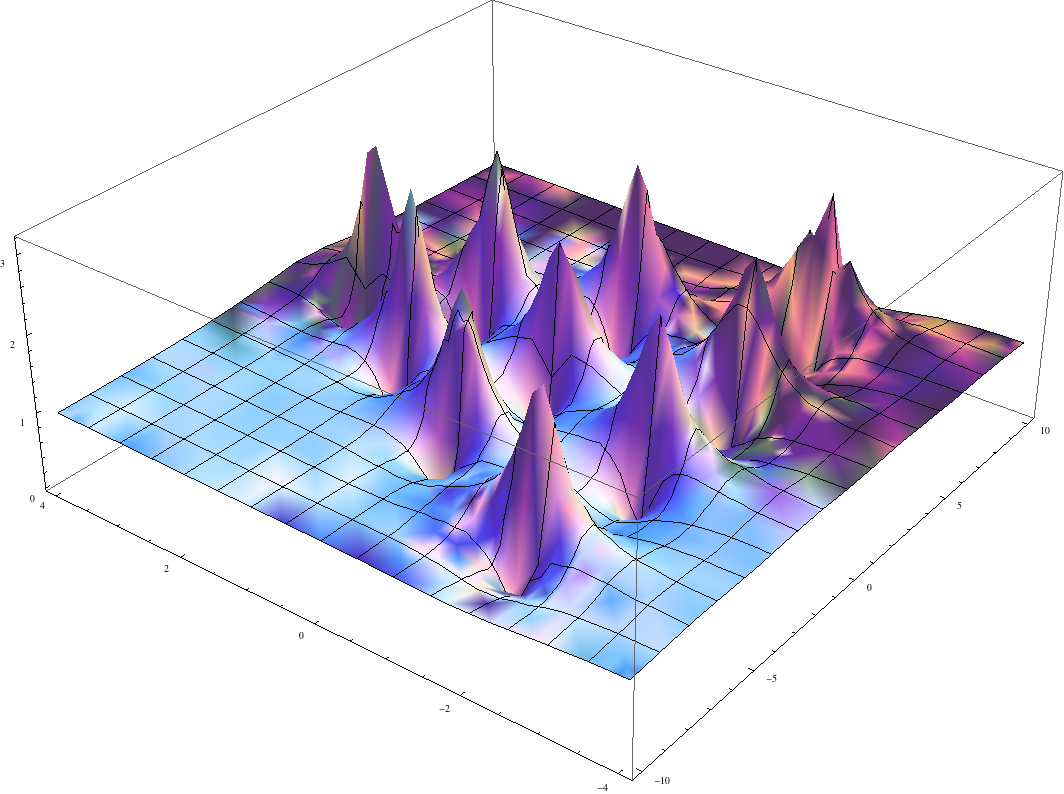
\includegraphics[width=200px]{4th_order_many_peaks.png}\\
Figure 11: Mathematica plot of 4rd order solution for $(a_3,a_5,a_7)=(25i/3,0,0)$.
\end{center}
\end{figure}
\vspace{-1mm}
}

\frame
{
\begin{figure}
\begin{center}
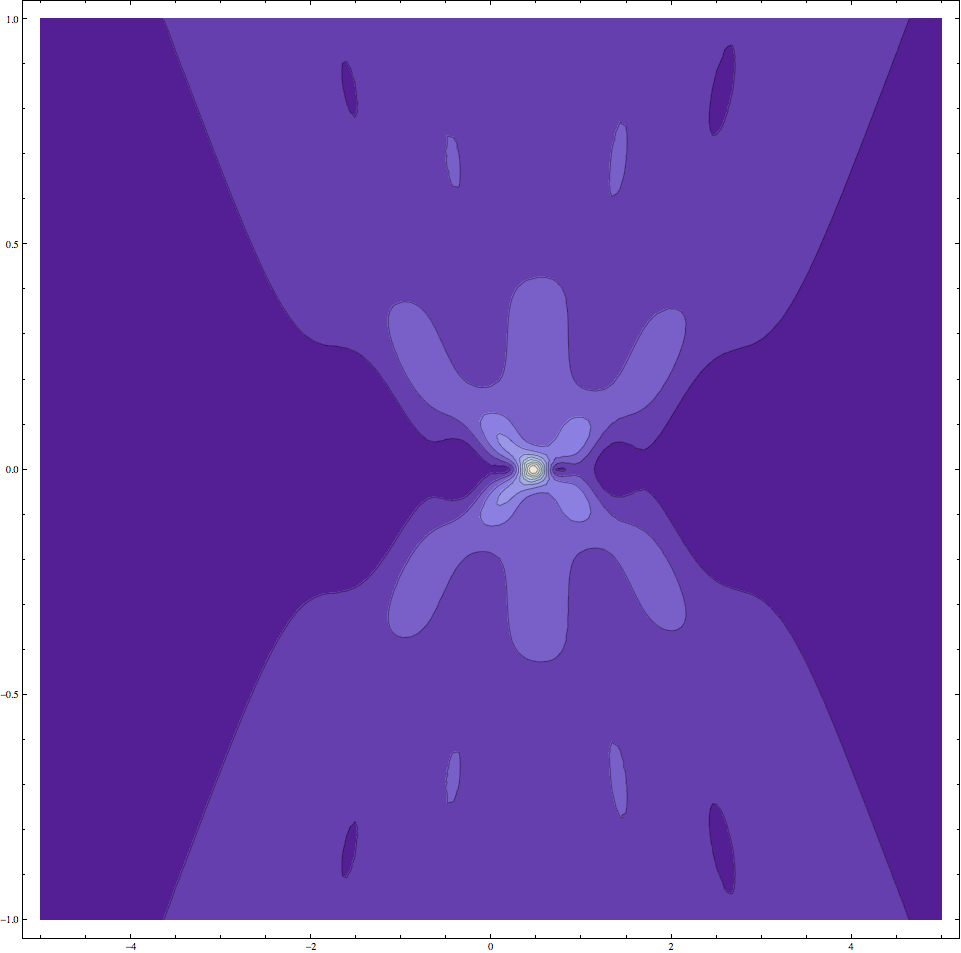
\includegraphics[width=150px]{4th_order_max_peak_contour.png}\\
Figure 12: Mathematica contour plot of 4rd order solution for $(a_3,a_5,a_7)=(-1/12,-1/240,0)$, which achieves a maximum amplitude of 9 also at $(1/2,0)$. 
\end{center}
\end{figure}
\vspace{-1mm}
}

\frame
{
\begin{figure}
\begin{center}
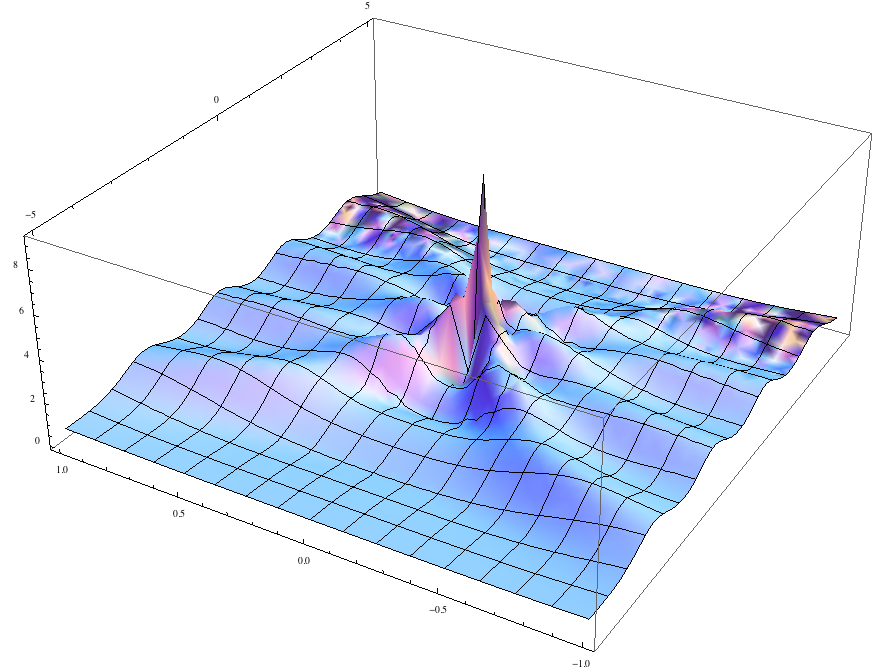
\includegraphics[width=200px]{4th_order_max_peak.png}\\
Figure 13: Mathematica plot of 4rd order solution for $(a_3,a_5,a_7)=(-1/12,-1/240,0)$.
\end{center}
\end{figure}
\vspace{-1mm}
}

\frame
{
\begin{figure}
\begin{center}
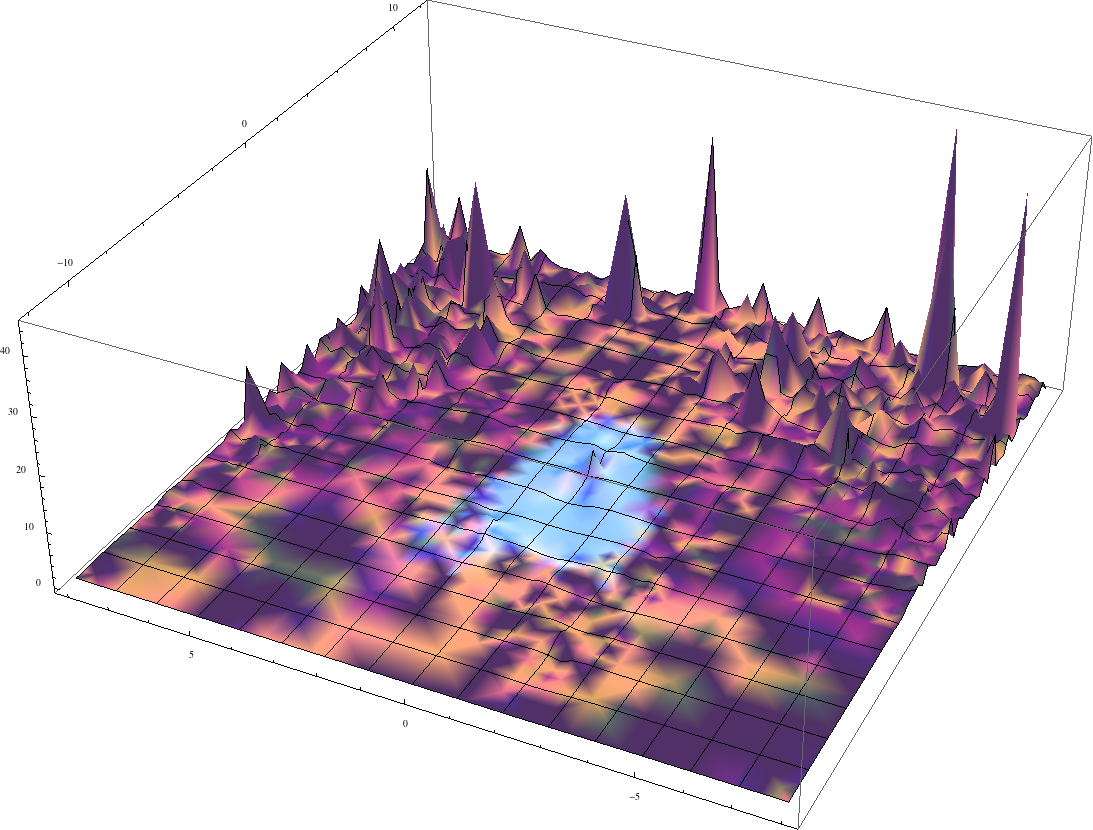
\includegraphics[width=200px]{5th_order_unstable.png}\\
Figure 14: Mathematica plot of 5th order solution for $(a_3,a_5,a_7,a_9)=(-1/12,-1/240,0,0)$ showing the extreme instability of such high order solutions. At $(x,t)=(1/2,0)$ this achieves a maximum amplitude of 11.
\end{center}
\end{figure}
\vspace{-1mm}
}

\frame
{
\begin{figure}
\begin{center}
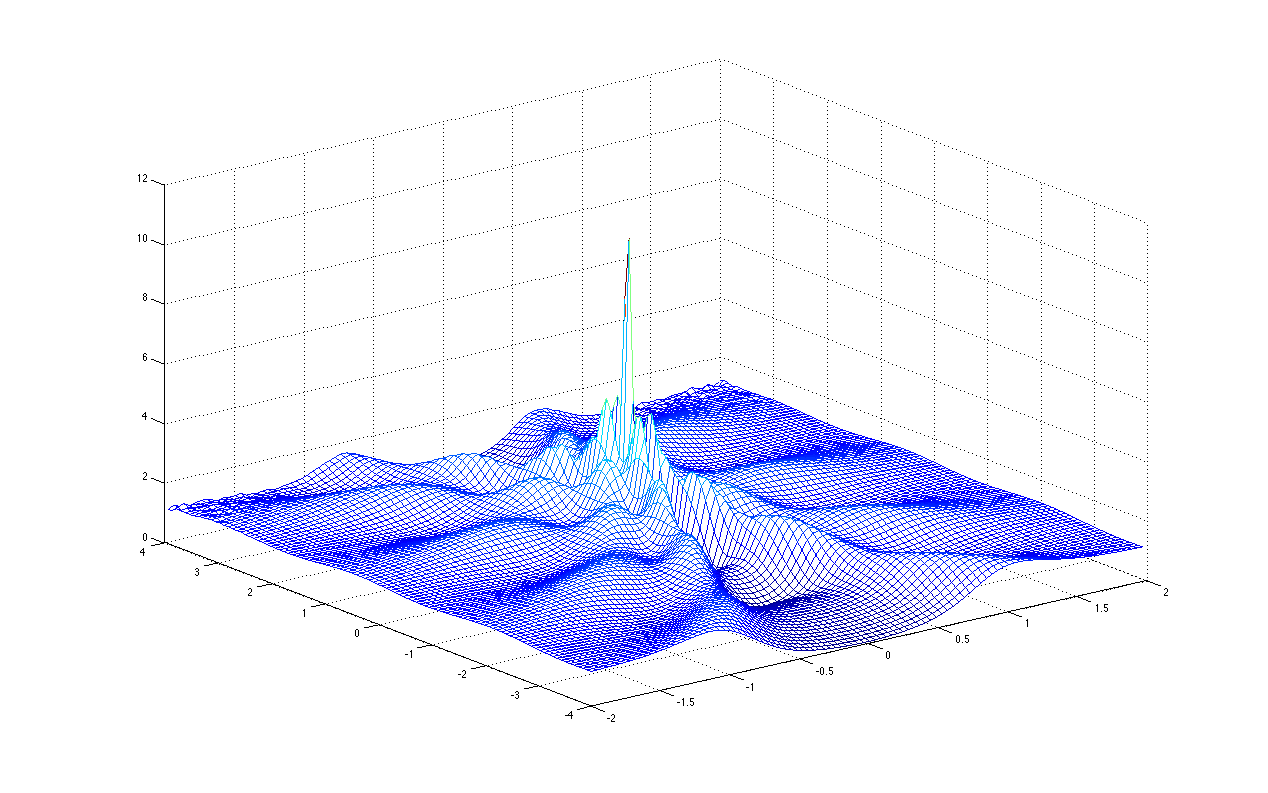
\includegraphics[width=200px]{matlab_5th_order_peak.png}\\
Figure 14: Matlab plot of 5th order solution for $(a_3,a_5,a_7,a_9)=(-1/12,-1/240,0,0)$ with higher accuracy, showing that Mathematica had numerical issues.
\end{center}
\end{figure}
\vspace{-1mm}
}


\end{document}